% =============================================================================
% COPYRIGHT AND DISCLAIMER
% =============================================================================
% This file is provided as a convenience template for competition participants.
% By using it, you accept full responsibility for compliance with all applicable
% copyright, licensing, and usage rules of the Association for Computing
% Machinery (ACM) and of any LaTeX packages you load (including, without
% limitation, the "acmart" document class and related ACM materials).
%
% Consult ACM's official publication, template, and copyright policies before
% using this setup for any purpose other than this competition. Do not assume
% that this template may be reused, redistributed, or submitted elsewhere
% without independently verifying ACM's current rules.
%
% Use of the "acmart" class, the "sigconf" option, or ACM-style formatting in
% this template does NOT mean that this report, this competition, its organizers,
% or any resulting PDF is sponsored, endorsed, affiliated with, or published by
% ACM. ACM trademarks and branding remain the property of ACM.
%
% Template packages live in preamble.tex.
% Citations live in main.bib. Edit this file with your paper content.
% =============================================================================

\documentclass[sigconf]{acmart}
% =============================================================================
% Template setup — participants normally do not edit this file.
% Author content belongs in main.tex; citations belong in main.bib.
% \documentclass lives in main.tex so Overleaf does not treat this file as root.
% =============================================================================

% --- Competition / non-ACM-submission friendly rights metadata -------------
\setcopyright{none}
\settopmatter{printacmref=false}
\acmConference[Kaggle Competition]{Filament Segmentation Challenge}{2026}{\href{https://www.kaggle.com/competitions/filament-segmentation-2026}{kaggle.com/competitions/filament-segmentation-2026}}
\acmBooktitle{Competition Report}
\acmDOI{}
\acmISBN{}

% --- Author guidance text --------------------------------------------------
% \guide{...} is gray italic while \guideStyletrue; omitted from the PDF if false.
% Flip the switch in main.tex after % =============================================================================
% Template setup — participants normally do not edit this file.
% Author content belongs in main.tex; citations belong in main.bib.
% \documentclass lives in main.tex so Overleaf does not treat this file as root.
% =============================================================================

% --- Competition / non-ACM-submission friendly rights metadata -------------
\setcopyright{none}
\settopmatter{printacmref=false}
\acmConference[Kaggle Competition]{Filament Segmentation Challenge}{2026}{\href{https://www.kaggle.com/competitions/filament-segmentation-2026}{kaggle.com/competitions/filament-segmentation-2026}}
\acmBooktitle{Competition Report}
\acmDOI{}
\acmISBN{}

% --- Author guidance text --------------------------------------------------
% \guide{...} is gray italic while \guideStyletrue; omitted from the PDF if false.
% Flip the switch in main.tex after % =============================================================================
% Template setup — participants normally do not edit this file.
% Author content belongs in main.tex; citations belong in main.bib.
% \documentclass lives in main.tex so Overleaf does not treat this file as root.
% =============================================================================

% --- Competition / non-ACM-submission friendly rights metadata -------------
\setcopyright{none}
\settopmatter{printacmref=false}
\acmConference[Kaggle Competition]{Filament Segmentation Challenge}{2026}{\href{https://www.kaggle.com/competitions/filament-segmentation-2026}{kaggle.com/competitions/filament-segmentation-2026}}
\acmBooktitle{Competition Report}
\acmDOI{}
\acmISBN{}

% --- Author guidance text --------------------------------------------------
% \guide{...} is gray italic while \guideStyletrue; omitted from the PDF if false.
% Flip the switch in main.tex after \input{preamble}.
%
% Do not use \guide{...} for \email{...}.
\usepackage{xcolor}
\newif\ifguideStyle
\guideStyletrue
\newcommand{\guide}[1]{%
  \ifguideStyle
    {\color{gray!65}\itshape #1}%
  \fi
}

% --- Math ------------------------------------------------------------------
% Do NOT load amssymb (or amsfonts): acmart already loads newtxmath, which
% defines the same symbols (e.g. \Bbbk) and causes a conflict on Overleaf.
% amsmath is already provided by acmart; mathtools extends it.
\usepackage{mathtools}

% --- Figures ---------------------------------------------------------------
% graphicx is already loaded by acmart
\usepackage{subcaption}

% --- Tables ----------------------------------------------------------------
% booktabs is already loaded by acmart
\usepackage{tabularx}
\usepackage{multirow}

% --- Bibliography style is set in main.tex (ACM-Reference-Format) ----------
.
%
% Do not use \guide{...} for \email{...}.
\usepackage{xcolor}
\newif\ifguideStyle
\guideStyletrue
\newcommand{\guide}[1]{%
  \ifguideStyle
    {\color{gray!65}\itshape #1}%
  \fi
}

% --- Math ------------------------------------------------------------------
% Do NOT load amssymb (or amsfonts): acmart already loads newtxmath, which
% defines the same symbols (e.g. \Bbbk) and causes a conflict on Overleaf.
% amsmath is already provided by acmart; mathtools extends it.
\usepackage{mathtools}

% --- Figures ---------------------------------------------------------------
% graphicx is already loaded by acmart
\usepackage{subcaption}

% --- Tables ----------------------------------------------------------------
% booktabs is already loaded by acmart
\usepackage{tabularx}
\usepackage{multirow}

% --- Bibliography style is set in main.tex (ACM-Reference-Format) ----------
.
%
% Do not use \guide{...} for \email{...}.
\usepackage{xcolor}
\newif\ifguideStyle
\guideStyletrue
\newcommand{\guide}[1]{%
  \ifguideStyle
    {\color{gray!65}\itshape #1}%
  \fi
}

% --- Math ------------------------------------------------------------------
% Do NOT load amssymb (or amsfonts): acmart already loads newtxmath, which
% defines the same symbols (e.g. \Bbbk) and causes a conflict on Overleaf.
% amsmath is already provided by acmart; mathtools extends it.
\usepackage{mathtools}

% --- Figures ---------------------------------------------------------------
% graphicx is already loaded by acmart
\usepackage{subcaption}

% --- Tables ----------------------------------------------------------------
% booktabs is already loaded by acmart
\usepackage{tabularx}
\usepackage{multirow}

% --- Bibliography style is set in main.tex (ACM-Reference-Format) ----------


% Guide styling: \guideStyletrue = show gray italic hints; \guideStylefalse = omit them
% \guideStyletrue
\guideStylefalse

% DRAFT: numbers still being measured are marked in red; remove this macro's uses before submitting.
\newcommand{\pending}[1]{\textcolor{red}{[#1]}}

\begin{document}

\title{A Full-Frame U-Net Ensemble and a Physically Motivated Pixel Analysis for Solar Filament Segmentation}
\subtitle{A Solution to the Solar Filament Segmentation Challenge 2026} % DO NOT CHANGE


\author{Jannat Samadov}
\affiliation{%
  \institution{Shamakhy Astrophysical Observatory named after N.~Tusi}
  \city{Shamakhy}
  \country{Azerbaijan}
}
\email{jannat.samadov@gmail.com}

\author{N. S. Dzhalilov}  % full first name to be confirmed
\affiliation{%
  \institution{Shamakhy Astrophysical Observatory named after N.~Tusi}
  \city{Shamakhy}
  \country{Azerbaijan}
}

\author{A. Habilov}  % full first name to be confirmed
\affiliation{%
  \institution{Baku State University}
  \city{Baku}
  \country{Azerbaijan}
}

\begin{abstract}
    This report describes our solution to the Solar Filament Segmentation Challenge~2026, a Kaggle competition on automatic segmentation of solar filaments in GONG H-$\alpha$ observations. The submitted pipeline averages the probability maps of ten full-frame U-Nets and of a vision-transformer segmenter, and keeps or discards each connected component with a learned rule that uses the heliographic position and orientation of the candidate. It reaches a panoptic quality (PQ) of 0.458 on held-out training photographs and 0.39 on the public test set. In parallel we describe each pixel of the solar disk by physical quantities (position on the Sun, time and station of the observation, contrast against the quiet Sun, the values of its neighbours, and the same solar point in other observations carried by differential rotation), in order to learn which physical information helps a classifier. We find that the classifier relies on darkness and on the elongated shape of the dark lane, and that the remaining errors are mainly faint filaments on which the experts themselves disagree.
\end{abstract}

\maketitle


% ==================================== %
%              INTRODUCTION            %
% ==================================== %
\section{Introduction}
    This report goes over the details of our submitted solution to the Solar Filament Segmentation Challenge~2026 \cite{filament-segmentation-2026}. The challenge, launched on July~10,~2026, is organized by the Earth-Space AI Research (ESAIR) Lab\footnote{\href{https://www.esairlab.com/home}{www.esairlab.com/}}. This challenge utilizes the MAGFiLO dataset for evaluation of the segmentation algorithms \cite{ahmadzadeh2024dataset}. Our work follows two lines. The first is a deep-learning pipeline that produced the submitted file. The second is a pixel-by-pixel analysis in which the input of a classifier is a table of physical quantities rather than an image; it asks which physical information (position, time, rotation, neighbourhood) helps beyond the brightness pattern itself. Throughout, we compare the models with the agreement between the experts, because many photographs were annotated by two or three experts independently. Preliminary results of this work were presented at a local conference in Azerbaijan.


% ==================================== %
%              METHODOLOGY             %
% ==================================== %
\section{Methodology}\label{sec:methodology}

\subsection{Data and sampling}
The training set contains 707 GONG H$\alpha$ photographs of $2048\times2048$ pixels. Of these, 411 were annotated by one expert, 145 by two and 151 by three, by 37 annotators in total. Filaments are thin: the median outline covers 1228 pixels and is about 8 pixels wide, so an error of two pixels on each edge already halves the intersection over union (IoU). We split the photographs into five folds, grouped by photograph. Fold~0 (566 training and 141 validation photographs) was used for development, and every model was then trained on all five folds, so that each training photograph has an out-of-fold prediction from a model that never saw it. Every threshold and cut applied to fold~0 is chosen \emph{nested}, i.e.\ on photographs other than the ones it is scored on.

\subsection{Segmentation networks}
\textbf{U-Nets.} The main model is a U-Net \cite{ronneberger2015unet} with an ImageNet-initialised ResNet-34 or ResNet-50 encoder \cite{he2016resnet}. It sees the full 2048-pixel grey frame and predicts one probability map. The target of a pixel is the fraction of the photograph's experts who drew it, so a pixel drawn by one of three experts counts as $1/3$. The loss is binary cross-entropy plus soft Dice on the solar disk. Training uses rotations by any angle, mirrors, and photometric changes (contrast, gamma, brightness, blur or sharpening, noise and JPEG re-compression) within the ranges we measured between GONG frames. At inference each model averages its predictions over the eight symmetries of the square (D4). Both encoders were trained on all five folds, which gives ten models.

\textbf{A vision-transformer segmenter.} To add a model whose errors differ from the U-Nets', we use the 24-block vision encoder of Qwen3-VL-2B \cite{qwen3vl2025} with a small convolutional branch and a mask decoder. It is first trained for one epoch on 2000 unlabelled GONG H$\alpha$ frames, with the U-Net ensemble's maps as targets, and then fine-tuned on the annotations. On fold~0 it reaches PQ~0.417, against 0.404 without the pre-training and 0.425 for a single ResNet-50 U-Net.

\textbf{YOLO11.} A YOLO11l-seg model \cite{yolo11} is trained per fold on the experts' outlines. Its own masks are weaker (PQ~0.385 on fold~0), so it is not used for the masks but as an independent opinion on each candidate (see below).

\subsection{Post-processing and selection rule}
The ten U-Net maps and the Qwen map are averaged, with weight 2/12 for the Qwen map. The mean map is thresholded at 0.65; pieces closer than 7 pixels are grouped into one filament (the grouping labels only the original pixels), and groups smaller than 350 pixels are dropped.

A candidate adds $\frac{1}{2}$ to the denominator of PQ (Eq.~\ref{eq:pq}) and adds its IoU to the numerator only if it is matched, so keeping it pays only if its probability of being matched times its expected IoU exceeds PQ$/2$. We therefore train gradient-boosted regression trees (scikit-learn HistGradientBoosting \cite{pedregosa2011scikit}, 300 trees of 15 leaves, learning rate 0.05) to predict the mean matched IoU of each candidate from 25 features: its area; the statistics of the probability inside it and on its rim; its elongation; its contrast against a surrounding ring; the threshold settings that produced it; its heliographic latitude and longitude from the central meridian (computed with the solar $B_0$ angle at the observation time); the orientation of its long axis ($\cos2\phi$, $\sin2\phi$); and four features measuring how strongly the YOLO11 models agree with it. The rule is trained on the out-of-fold candidates of all 707 photographs, and candidates with a predicted IoU below 0.18 are discarded. The masks are encoded as COCO run-length strings. Fig.~\ref{fig:pipeline} summarises the pipeline, and Fig.~\ref{fig:test} shows the submitted masks on a test photograph.

\begin{figure}[t]
  \centering
  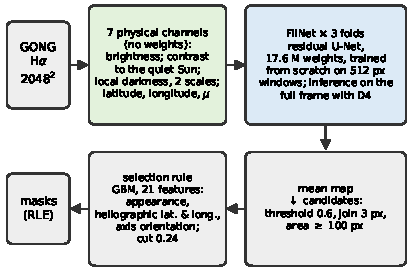
\includegraphics[width=\columnwidth]{fig_pipeline.pdf}
  \caption{The submitted pipeline.}
  \label{fig:pipeline}
\end{figure}

\begin{figure*}[t]
  \centering
  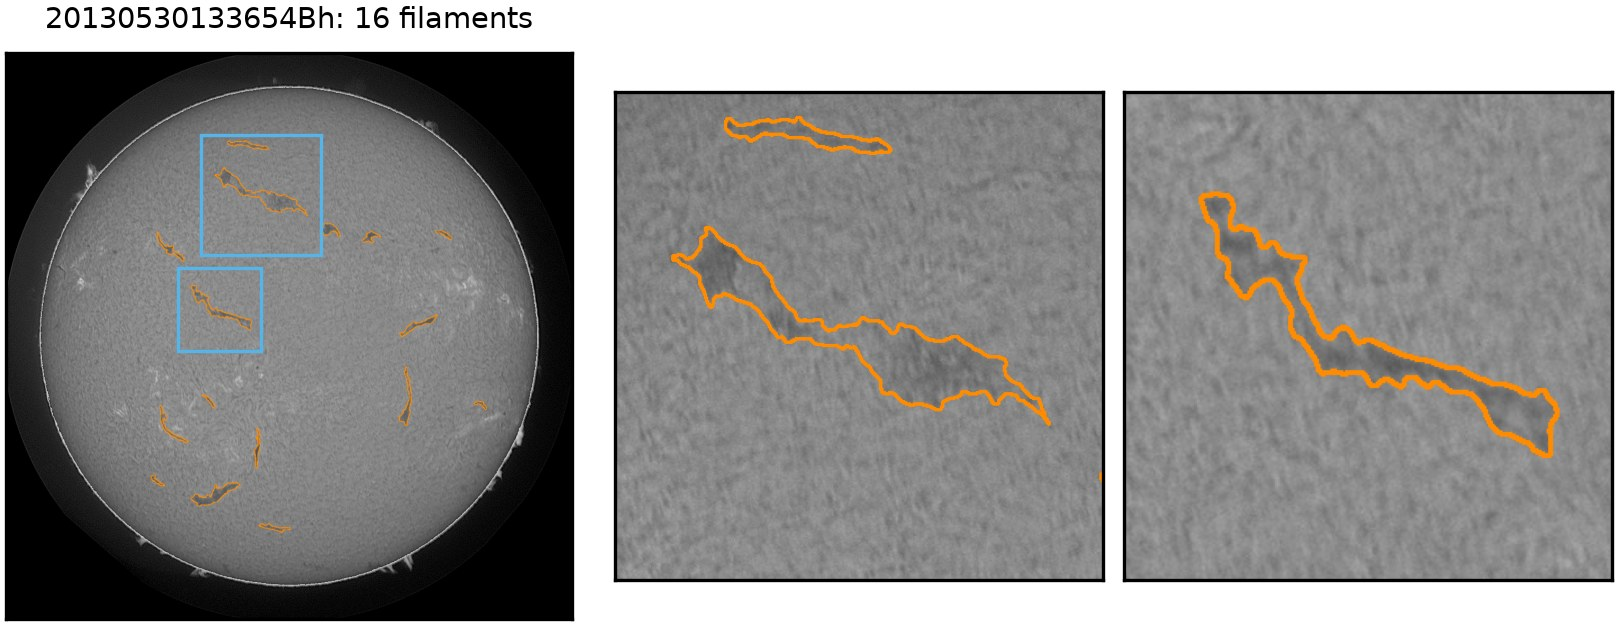
\includegraphics[width=0.92\textwidth]{fig_test.jpg}
  \caption{The submitted masks (orange) on the test photograph with the most filaments, 20130530133654Bh: the full disk and two close-ups.}
  \label{fig:test}
\end{figure*}

\subsection{Physically motivated pixel analysis}
In this line of work each disk pixel is one row of a table, and a random forest \cite{breiman2001random} (100 trees, each on 10\% of the rows, at least 50 rows per leaf) classifies it as filament or background. The first table has 35 columns in four groups:
\begin{itemize}
\item \emph{position on the Sun}: image position, distance from the disk centre, $\mu$, heliographic latitude and longitude, and the differential rotation rate at that latitude;
\item \emph{time and station}: $B_0$, the date as a phase of the solar cycle, the hour and the GONG station;
\item \emph{darkness}: the brightness, its ratio to the disk median and to the quiet-Sun brightness at the same $\mu$ (limb darkening removed), this contrast smoothed at four scales, and its ratio to the mean of the neighbourhood at four radii;
\item \emph{shape}: the eigenvalues of the Hessian at three scales, which respond to a dark lane, and the lane's orientation.
\end{itemize}
We then extended the table in two ways. First, every row also holds the contrast and the position of each of the 440 pixels within 12 pixels of it, so that the classifier can see that a filament pixel has similar neighbours (1358 columns). Training photographs enter five times: as they are, and with only their contrast, only their sharpness, only their brightness, or all three changed; rotations are not used, so that the position columns stay physical. Second, we add the Sun's rotation: the displacement of the pixel per hour from differential rotation \cite{snodgrass1990rotation}, and, for each of six time windows (0--24, 24--48 and 48--84 hours before and after the observation), the nearest other photograph, in which the same solar point is located by differential rotation and the contrast within 6 pixels of it is read.

The same information is given to a per-pixel neural network (PixNet): a stack of twelve dilated $3\times3$ convolutions with ReLU, which sees about 260 pixels around each pixel, with the photograph-level quantities entering every layer through feature-wise modulation \cite{perez2018film}. Variants receive the 35 columns as extra input channels, and the other photographs, carried to the observation time by differential rotation, as further channels.


% ==================================== %
%              EVALUATION              %
% ==================================== %
\section{Evaluation}\label{sec:evaluation}

\subsection{Strategy}
A prediction $p$ matches an annotation $g$ if IoU$(p,g)>0.5$, and
\begin{equation}\label{eq:pq}
\mathrm{PQ}=\frac{\sum_{(p,g)\in\mathrm{TP}}\mathrm{IoU}(p,g)}{|\mathrm{TP}|+\frac12|\mathrm{FP}|+\frac12|\mathrm{FN}|},
\end{equation}
where the counts are pooled over every annotation set of every photograph \cite{kirillov2019panoptic}. Our scorer reproduces the organisers' counts exactly. With 141 validation photographs the sampling noise of PQ is about $\pm0.02$, so we report differences between models with 95\% bootstrap intervals over photographs. As a reference we score one expert against another on the same photographs: two experts agree at PQ~0.348.

\subsection{Results}
Table~\ref{tab:dev} shows how the score developed. Our first approach (a spine and half-width network with physical input channels) reached 0.29 on the test set. The full-frame U-Net with soft targets raised this to 0.36, the ensemble and the selection rule to 0.38, and the second model family to 0.39. Table~\ref{tab:abl} gives the contribution of each component. Fig.~\ref{fig:morph} compares our filaments with the experts' on validation photographs.

\begin{table}[t]
\caption{Development: validation PQ on fold~0 (nested) and public test PQ.}
\label{tab:dev}
\centering\small
\begin{tabular}{@{}lcc@{}}
\toprule
Model & Val. & Test \\
\midrule
Spine/half-width U-Net, physical channels & 0.355 & 0.29 \\
Full-frame U-Net ResNet-50, soft target, D4 & 0.434 & 0.36 \\
Ensemble + selection rule & 0.440 & 0.38 \\
10 fold models + rule with heliographic features & 0.452 & 0.38 \\
+ Qwen segmenter map + YOLO11 features (submitted) & \textbf{0.458} & \textbf{0.39} \\
\bottomrule
\end{tabular}
\end{table}

\begin{table}[t]
\caption{Effect of single components: $\Delta$PQ with 95\% bootstrap intervals. OOF = out-of-fold on all 707 photographs; ens.\ = fold-0 ensemble.}
\label{tab:abl}
\centering\small
\begin{tabular}{@{}lc@{}}
\toprule
Change & $\Delta$PQ \\
\midrule
D4 symmetry averaging (OOF) & $+0.005\ [+0.002,\,+0.009]$ \\
ResNet-50 + ResNet-34 vs.\ ResNet-50 (OOF) & $+0.004\ [+0.001,\,+0.007]$ \\
Selection rule (OOF) & $+0.012\ [+0.008,\,+0.017]$ \\
Heliographic features in the rule (ens.) & $+0.005\ [+0.000,\,+0.010]$ \\
Qwen map + YOLO11 features (ens.) & $+0.006\ [+0.001,\,+0.012]$ \\
\midrule
Neighbouring frames by differential rotation (OOF) & $-0.002\ [-0.004,\,-0.000]$ \\
Pixel random forest added to the ensemble (ens.) & $-0.001\ [-0.007,\,+0.005]$ \\
\bottomrule
\end{tabular}
\end{table}

\begin{figure}[t]
  \centering
  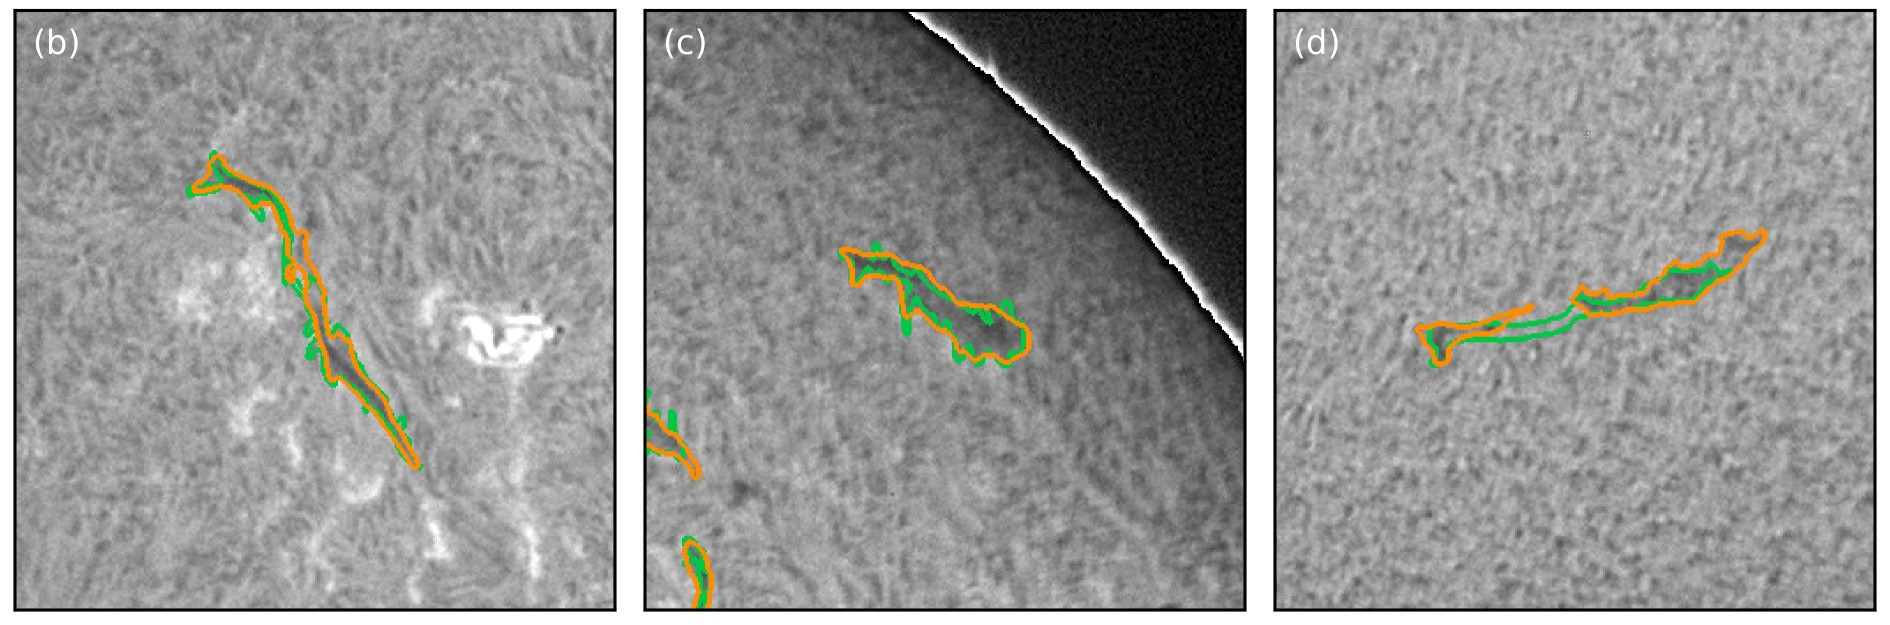
\includegraphics[width=\columnwidth]{fig_morph.jpg}
  \caption{Validation photographs not seen in training: expert outlines (green) and the U-Net ensemble's filaments (orange).}
  \label{fig:morph}
\end{figure}

\textbf{Pixel level.} Against the union of the experts, the submitted map labels the pixels of the 141 validation photographs with precision 0.763, recall 0.669 and F1 0.713. One expert scored in the same way against the other experts reaches F1 0.651, so at the pixel level the model agrees with the experts better than they agree with each other.

\textbf{Physical pixel analysis.} The 35-column random forest alone finds fewer than half of the filament pixels (recall 0.415, F1 0.543). When the U-Net probability is added as a column, the forest ranks pixels best of all models (area under the ROC curve 0.990), but its best F1 (0.711) equals that of its U-Net input (0.714). Shuffling one group of columns at a time shows what the forest uses: the darkness columns raise the log-loss by 0.154, the shape columns by 0.036, position, time and station together by 0.017, and the photograph statistics by 0.003. The station, the year and the hour are almost unused: a filament is recognised by its darkness and its elongated shape, not by where or when it was observed. \pending{Results of the 1358-column neighbour table, the rotation columns and PixNet with the table and rotation channels.} PixNet without these channels stopped at PQ~0.38 on fold~0.

\subsection{Strengths, weaknesses and possible improvements}
The pipeline's strengths are that every component was checked out-of-fold with intervals, that the geometric features add physical information the image lacks, and that the masks follow the shape of the dark lane closely (Fig.~\ref{fig:test}). Its main weakness is shown in Fig.~\ref{fig:ceiling}. On fold~0, replacing the learned rule with a perfect filter on the same candidates would raise PQ only from 0.458 to 0.500. Perfect pixels, taken as the experts' majority, would give 0.769, but they are built from the same experts who score them, so this is a ceiling rather than a target. The ensemble finds 97\% of the filaments that every other expert of the same photograph also drew, but only 43\% of those that no other expert drew, and 55\% of the faintest fifth of the filaments against 98\% of the darkest fifth.

\begin{figure}[t]
  \centering
  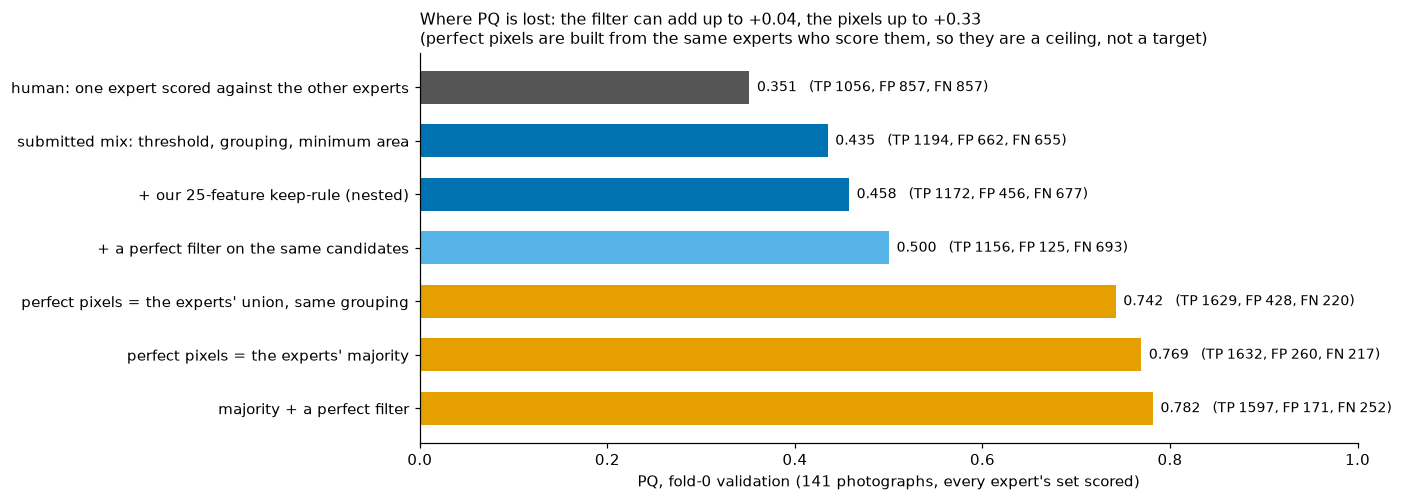
\includegraphics[width=\columnwidth]{fig_ceiling.png}
  \caption{Fold-0 PQ from one expert scored against the others, through our pipeline, up to a perfect filter and to perfect pixels.}
  \label{fig:ceiling}
\end{figure}

These numbers point to the annotations. For 17\% of the filaments a second expert drew nothing, and small filaments are the most disputed: the second expert misses 41\% of the filaments smaller than 500 pixels but 9\% of those larger than 2000 pixels. The outlines themselves are well placed (only 2 of 8177 are not darker than their surroundings), so the experts disagree about \emph{whether} a faint structure is a filament rather than about \emph{where} it is. The test set appears to be annotated more sparsely: removing the weakest 24\% of our test filaments did not change the public score, while validation predicted a loss of 0.03. All our models, like the public solutions of other teams, score 0.06--0.07 lower on the test set than on validation.

Several ideas did not help and are reported for completeness: Mask R-CNN with standard anchors (which reach IoU~$\geq0.7$ with only a third of the filament boxes), self-training, pre-training the encoder on unlabelled GONG frames (0.35 on the test set), a vision-language model judging each candidate, and carrying candidates to neighbouring frames, which reached only 28\% of the candidates. Improvements are most likely to come from modelling the reliability of individual annotators \cite{tanno2019learning}, which requires knowing who annotated each test photograph, and from using a second observation of the same filament whenever one exists.


% ==================================== %
%            ACKNOWLEDGMENT            %
% ==================================== %
\section{Acknowledgment}\label{sec:acknowledgment}
    % Do not change
    The organization of the Filament Segmentation Challenge 2026 is partially supported by the U.S. National Science Foundation (NSF) under Grant No. 2209912 and 2433781, directorate for Computer and Information Science and Engineering (CSE), and Office of Advanced Cyberinfrastructure (OAC), and Grant No. 2511630, AST Division Of Astronomical Sciences and MPS Directorate for Mathematical and Physical Sciences.

    The Filament Segmentation Challenge 2026 is sponsored by the U.S. National Science Foundation (NSF) National Solar Observatory (NSO).

    This work utilizes GONG data obtained by the NSO Integrated Synoptic Program, managed by the National Solar Observatory, which is operated by the Association of Universities for Research in Astronomy (AURA), Inc. under a cooperative agreement with the National Science Foundation and with contribution from the National Oceanic and Atmospheric Administration. The GONG network of instruments is hosted by the Big Bear Solar Observatory, High Altitude Observatory, Learmonth Solar Observatory, Udaipur Solar Observatory, Instituto de Astrofísica de Canarias, and Cerro Tololo Interamerican Observatory.

\bibliographystyle{ACM-Reference-Format}
\bibliography{main}

\end{document}
